\chapter{Introduction}
Lorem ipsum dolor sit amet, consetetur sadipscing elitr, sed diam nonumy eirmod tempor invidunt ut labore et dolore magna aliquyam erat, sed diam voluptua. At vero eos et accusam et justo duo dolores et ea rebum. \cite{Abedon2003}

{\color{red}some colored text}

\section{First Section}
Lorem ipsum dolor sit amet, consetetur sadipscing elitr, sed diam nonumy eirmod tempor invidunt ut labore et dolore magna aliquyam erat, sed diam voluptua. At vero eos et accusam et justo duo dolores et ea rebum. Stet clita kasd gubergren, no sea takimata sanctus est Lorem ipsum dolor sit amet. Lorem ipsum dolor sit amet, consetetur sadipscing elitr, sed diam nonumy eirmod tempor invidunt ut labore et dolore magna aliquyam erat, sed diam voluptua. At vero eos et accusam et justo duo dolores et ea rebum. Stet clita kasd gubergren, no sea takimata sanctus est Lorem ipsum dolor sit amet. \cite{Goossens1993}

\section{Embedding code samples}
Code listings can be modified with \textbackslash lstset (see .sty file). Code samples can either be embedded directly inline, as displayed in listing \ref{lst:python_inline_sample}.
% Also see: https://en.wikibooks.org/wiki/LaTeX/Source_Code_Listings.

%\begin{minipage}{\linewidth}
\begin{lstlisting}[caption={Python hello function.},captionpos=b,language=python,label=lst:python_inline_sample]
# prints hello
def hello(name):
    print('Hello, {}'.format(name))
\end{lstlisting}
%\end{minipage}
%
Or by including a file like so, see \ref{lst:python_file_sample}. To avoid page breaks within code snippets, use the minipage environment. This also smallers the code area which means it's aligning the line numbers with the "normal" text.

%\begin{minipage}{\linewidth}
\lstinputlisting[caption={Python hey function.},captionpos=b,label=lst:python_file_sample,language=python]{src/sample.py}
%\end{minipage}

\section{Images and labeling}
In order to include images, you need the graphicx package. The environment \textbackslash begin\{figure\} allows to label images. \textbackslash centering centers the image horizontally. \textbackslash includegraphics embeds the image (see figure \ref{fig:lighthouse}). 

\begin{figure}[h]
\centering
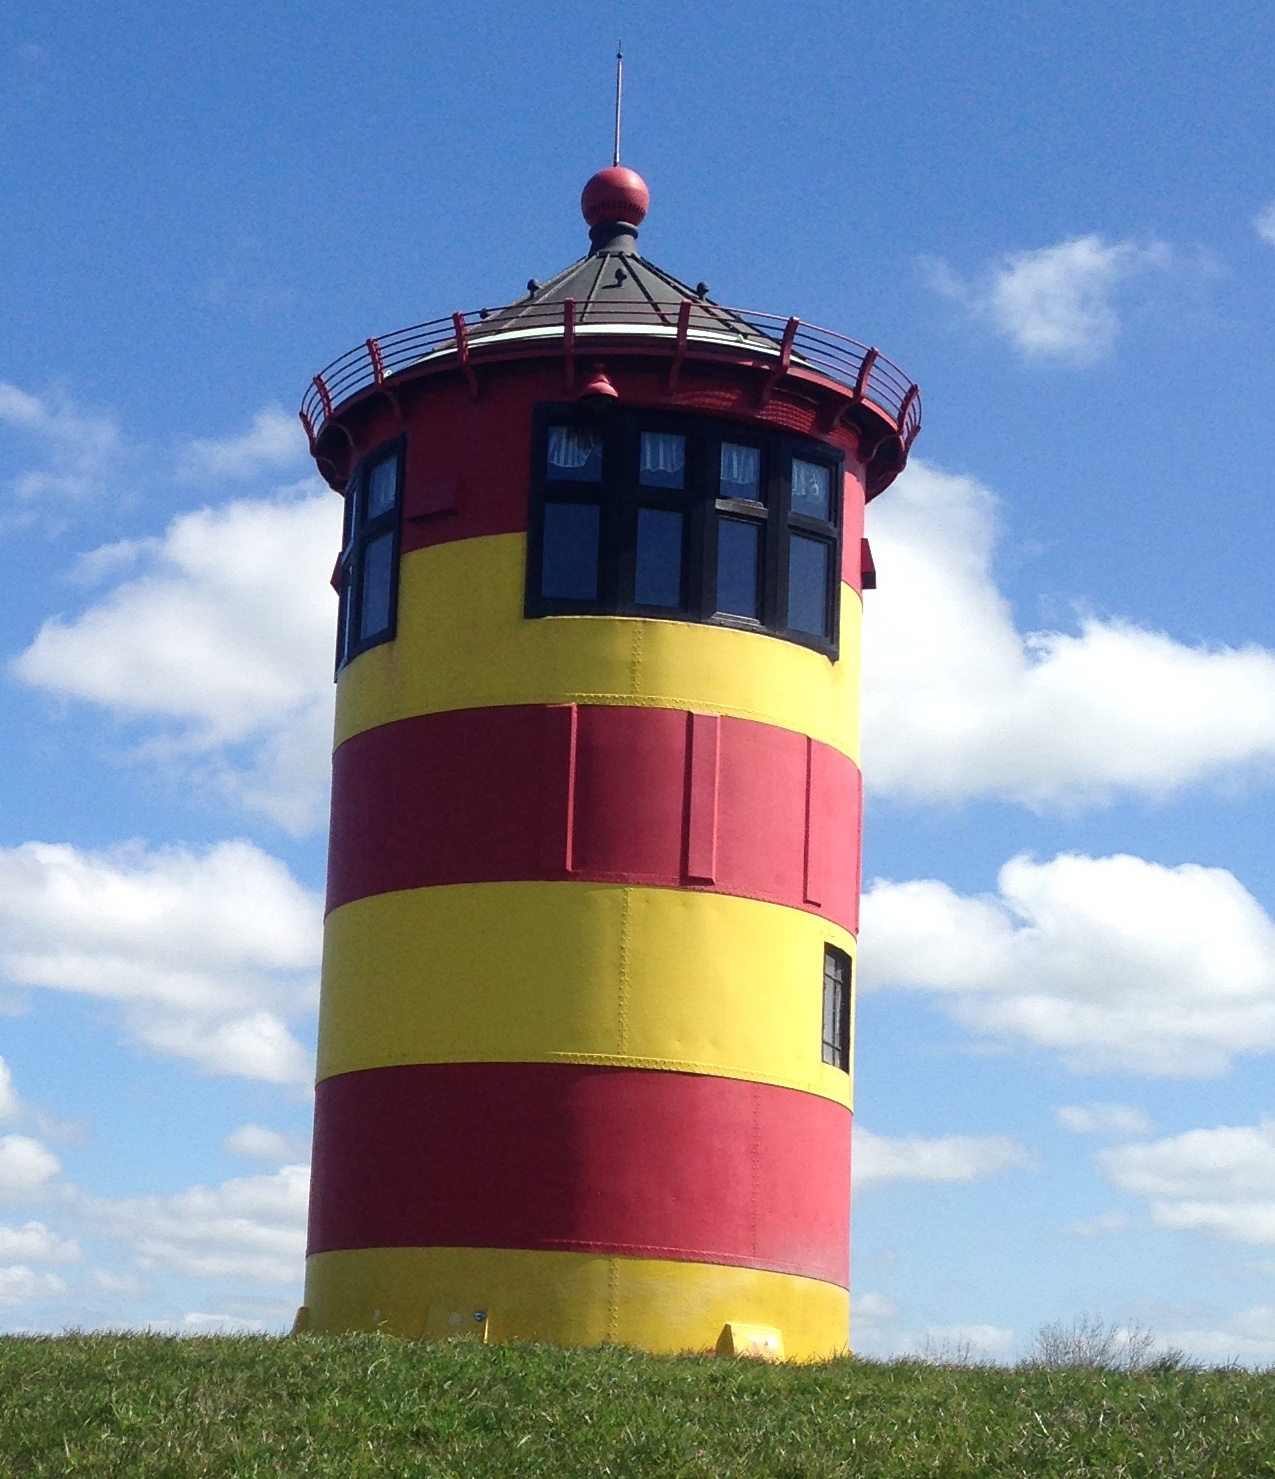
\includegraphics[width=0.5\textwidth]{img/lighthouse.jpg}
\caption{A red and yellow lighthouse.}
\label{fig:lighthouse}
\end{figure}

\section{Tables}
The tabular environment can be used to create tables. The second argument contains the table spec, which specifies the alignment of each column and the vertical lines. Besides some other specs, the table \ref{table:specs}.

\begin{table}[h]
\centering
\begin{tabular}{| l | l |}
\hline
l & left-justified column \\ \hline
c & centered column \\ \hline
r & right-justified column\\ 
\hline
\end{tabular}
\caption{table specs.}
\label{table:specs}
\end{table}

Another example of a table using different alignments and alternating row colors, see table \ref{table:alignment}. 

\begin{table}[ht]
\rowcolors{1}{gray!25}{white}
\centering
\begin{tabular}{ l | r | c }
\rowcolor{gray!40}
left & right & center  \\ \hline\hline
1 & 2 & 3 \\ \hline
11 & 22 & 33 \\ \hline
11,1 & 22,2 & 33,3 \\ 
\end{tabular}
\caption{table alignments and alternating row colors.}
\label{table:alignment}
\end{table} 

% https://en.wikibooks.org/wiki/LaTeX/Tables
For further possibilities to modify tables, see WikiBooks resource.

\section{Mathematical expressions}
Mathematical equations and expressions can be displayed inline using the math environment or its shorthand \textbackslash(...\textbackslash) (e.g. \( 3*x = 7 \)). Or as displayed formulas using either the displaymath environment (shorthand \textbackslash[...\textbackslash]) or the equation environment, which automatically numbers the equation.

\begin{figure}[h]
\[ \int_0^\infty \mathrm{e}^{-x}\,\mathrm{d}x \]
\caption{Equation using the displaymath environment shorthand.}
\label{fig:integral}
\end{figure}

The equation \ref{fig:numbered} is numbered and labeled in order to refer to it. This is the recommended style.

\begin{equation}
\lim_{x \to \infty} \exp(-x) = 0
\label{fig:numbered}
\end{equation}












